\documentclass[11pt,a4paper]{article}

\usepackage[utf8]{inputenc}
\usepackage[T1]{fontenc}
\usepackage{geometry}
\usepackage{titlesec}
\usepackage{graphicx}
\usepackage{float}
\usepackage{xcolor}
\usepackage{listings}
\usepackage{hyperref}
\usepackage{enumitem}

\geometry{margin=2.5cm}

\hypersetup{
    colorlinks=true,
    linkcolor=blue,
    urlcolor=blue
}

\titleformat{\section}
{\large\bfseries}
{\thesection.}{0.5em}{}

\titleformat{\subsection}
{\normalsize\bfseries}
{\thesubsection.}{0.5em}{}

\definecolor{codebg}{rgb}{0.95,0.95,0.95}

\lstset{
    backgroundcolor=\color{codebg},
    basicstyle=\ttfamily\small,
    frame=single,
    breaklines=true,
    columns=fullflexible
}

\begin{document}

\begin{titlepage}
    \centering

    \vspace*{3cm}

    {\Huge \textbf{Infrastructure Monitoring with Zabbix}}\\[1cm]

    {\Large Server Engineering Labs}\\[2cm]

    \textbf{Author:}\\
    Laura Ortiz Moreno\\[1cm]

    \textbf{Topics Covered:}
    \begin{itemize}[leftmargin=4cm]
        \item Infrastructure monitoring
        \item Zabbix server deployment
        \item Zabbix Agent2 configuration
        \item MariaDB integration
        \item Apache frontend configuration
        \item Linux service monitoring
    \end{itemize}

    \vfill

    \textbf{Environment:}\\
    Debian Monitoring Server\\
    Rocky Linux Client VM\\
    Virtualized lab environment

    \vspace{1cm}

\end{titlepage}

\tableofcontents
\newpage

\section{Introduction}

This report documents the deployment and configuration of a monitoring infrastructure using Zabbix.

The laboratory focused on:
\begin{itemize}
    \item Installing Zabbix Server
    \item Configuring MariaDB integration
    \item Deploying the Zabbix web frontend
    \item Configuring Zabbix Agent2
    \item Monitoring remote Linux hosts
    \item Testing alerts and service availability
\end{itemize}

The monitoring environment was deployed using Debian as the monitoring server and Rocky Linux as the monitored client system.

\section{Environment Preparation}

Before deploying Zabbix, network connectivity between machines was verified.

Useful commands included:

\begin{lstlisting}[language=bash]
ping <host>
ssh user@host
\end{lstlisting}

Firewall rules were also validated to allow monitoring traffic.

Required ports included:
\begin{itemize}
    \item 10051/tcp — Zabbix Server
    \item 10050/tcp — Zabbix Agent
    \item 80/tcp — Apache Web Interface
    \item Custom SSH port for administration
\end{itemize}

\begin{figure}[H]
    \centering
    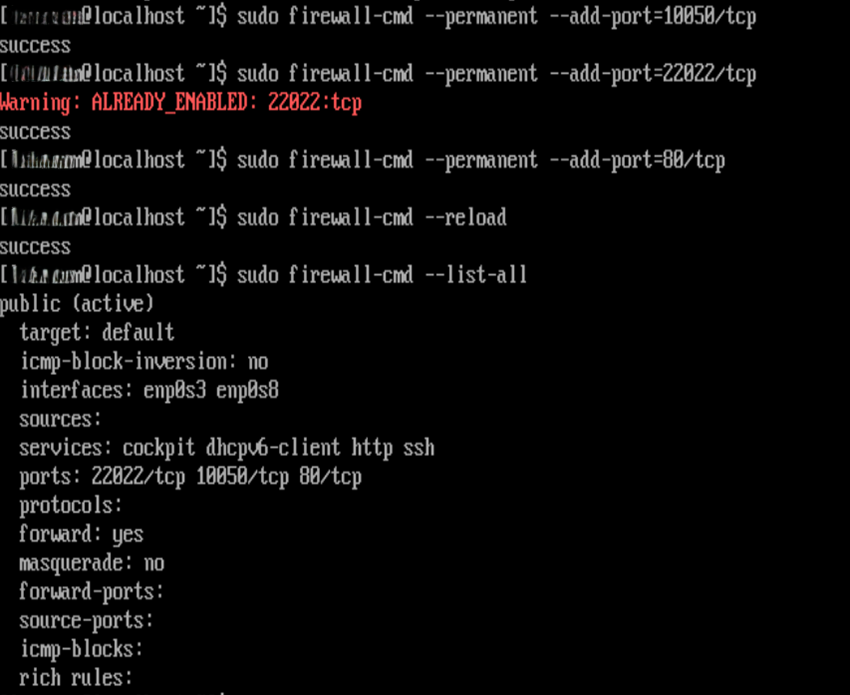
\includegraphics[width=0.88\textwidth]{images/zabbix/firewall-rules.png}
    \caption{Firewall configuration allowing monitoring, SSH, and web service traffic required by the Zabbix infrastructure.}
\end{figure}

\section{Installing Zabbix Server}

The official Zabbix repository was added to the Debian system.

Example:

\begin{lstlisting}[language=bash]
wget https://repo.zabbix.com/...
sudo dpkg -i zabbix-release.deb
sudo apt update
\end{lstlisting}

The required packages were then installed:

\begin{lstlisting}[language=bash]
sudo apt install zabbix-server-mysql \
                 zabbix-frontend-php \
                 zabbix-apache-conf \
                 zabbix-sql-scripts \
                 zabbix-agent2
\end{lstlisting}

\section{MariaDB Database Configuration}

Zabbix requires a relational database backend.

A database and dedicated user were created:

\begin{lstlisting}[language=SQL]
CREATE DATABASE zabbix;
CREATE USER 'zabbix'@'localhost'
IDENTIFIED BY 'secure_password';

GRANT ALL PRIVILEGES ON zabbix.*
TO 'zabbix'@'localhost';

FLUSH PRIVILEGES;
\end{lstlisting}

The initial schema was imported:

\begin{lstlisting}[language=bash]
zcat /usr/share/zabbix-sql-scripts/mysql/server.sql.gz \
| mysql -u zabbix -p zabbix
\end{lstlisting}

\section{Zabbix Server Configuration}

The Zabbix server configuration file was edited:

\begin{lstlisting}
/etc/zabbix/zabbix_server.conf
\end{lstlisting}

The database password parameter was configured:

\begin{lstlisting}
DBPassword=secure_password
\end{lstlisting}

The service was restarted afterward:

\begin{lstlisting}[language=bash]
sudo systemctl restart zabbix-server
\end{lstlisting}

\begin{figure}[H]
    \centering
    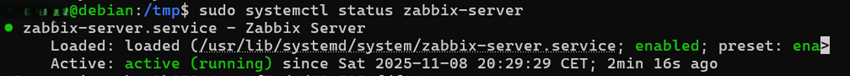
\includegraphics[width=0.88\textwidth]{images/zabbix/zabbix-server-running.png}
    \caption{Zabbix server service successfully running after backend configuration and initialization.}
\end{figure}

\section{Apache Frontend Configuration}

The Apache frontend was configured to serve the Zabbix web interface.

Apache configuration was validated:

\begin{lstlisting}[language=bash]
sudo systemctl status apache2
\end{lstlisting}

The PHP timezone was also configured:

\begin{lstlisting}
date.timezone = Europe/Madrid
\end{lstlisting}

Apache was restarted after applying changes:

\begin{lstlisting}[language=bash]
sudo systemctl restart apache2
\end{lstlisting}

\subsection{UTF-8 Locale Troubleshooting}

During deployment, locale issues affected the frontend checks.

The system locale was updated to use UTF-8 encoding:

\begin{lstlisting}[language=bash]
sudo locale-gen en_US.UTF-8
sudo update-locale
\end{lstlisting}

Apache environment variables were adjusted accordingly.

\begin{figure}[H]
    \centering
    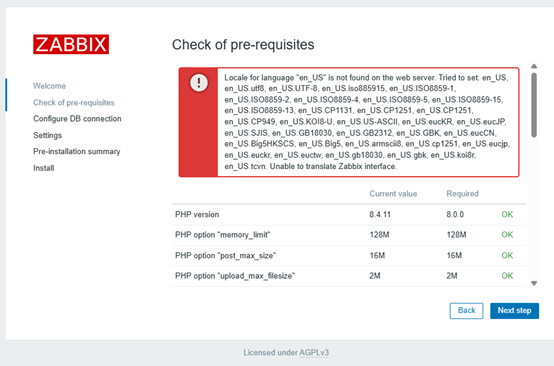
\includegraphics[width=0.78\textwidth]{images/zabbix/frontend-prerequisites.png}
    \caption{Zabbix frontend prerequisite validation highlighting locale configuration checks during deployment.}
\end{figure}

\section{Installing and Configuring Zabbix Agent2}

The monitored Rocky Linux machine was configured with Zabbix Agent2.

Installation:

\begin{lstlisting}[language=bash]
sudo dnf install zabbix-agent2
\end{lstlisting}

The agent configuration file was edited:

\begin{lstlisting}
/etc/zabbix/zabbix_agent2.conf
\end{lstlisting}

Important parameters:

\begin{lstlisting}
Server=<zabbix_server_ip>
ServerActive=<zabbix_server_ip>
Hostname=rocky-monitor-node
\end{lstlisting}

The service was enabled and started:

\begin{lstlisting}[language=bash]
sudo systemctl enable zabbix-agent2
sudo systemctl restart zabbix-agent2
\end{lstlisting}

\section{Frontend Host Registration}

The Rocky Linux machine was added as a monitored host in the Zabbix frontend.

The following information was configured:
\begin{itemize}
    \item Hostname
    \item Agent IP address
    \item Monitoring templates
    \item Availability checks
\end{itemize}

Monitoring metrics became visible after successful registration.

\begin{figure}[H]
    \centering
    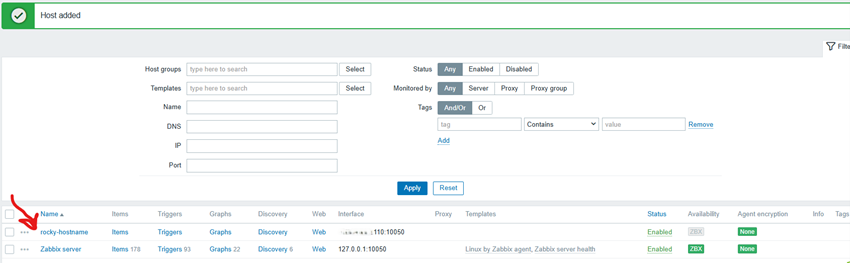
\includegraphics[width=0.95\textwidth]{images/zabbix/host-added.png}
    \caption{Successful registration of the monitored host in the Zabbix frontend interface.}
\end{figure}

\section{Monitoring Validation}

Several tests were performed to validate the monitoring infrastructure:
\begin{itemize}
    \item Service availability checks
    \item Agent communication validation
    \item CPU and memory monitoring
    \item Trigger and alert simulation
\end{itemize}

The Zabbix dashboard successfully displayed system metrics from the monitored host.

\section{Challenges Encountered}

Several issues appeared during deployment:
\begin{itemize}
    \item Database authentication problems
    \item Apache frontend configuration issues
    \item UTF-8 locale incompatibilities
    \item Firewall restrictions
    \item Agent communication failures
\end{itemize}

Troubleshooting these issues provided valuable practical experience in monitoring infrastructure administration.

\section{Conclusion}

This laboratory introduced the deployment of a complete infrastructure monitoring solution using Zabbix.

The exercises demonstrated:
\begin{itemize}
    \item Monitoring server deployment
    \item Agent-based infrastructure monitoring
    \item Database integration
    \item Frontend configuration
    \item Linux service administration
    \item Monitoring validation and troubleshooting
\end{itemize}

These concepts are highly relevant in infrastructure engineering, DevOps, system administration, and production monitoring environments.

\end{document}